\section{Introduction}
\label{sec:int}
In this project, we will learn how to measure the performance of an operating system using various user- and system-level operations. Based on prior knowledge of hardware performance as well as measured software behavior, we will approximately estimate the overhead at the operating system level of the whole system hardware/software stack. We select a well-known multi-user time-sharing operating system, Ubuntu 14.04.1 LTS (desktop) \footnote{http://www.ubuntu.com/download/desktop}, as our experiment platform. This is a long time supported Linux distribution with stable performance and reliable system functions. Our hardware platform is a $Lenovo Y400$  workstation equipped with an $Intel$  $4 cores$ processor. The experimental results indicate that our system configuration is trustable, it also helps us understand the underlying mechanisms of the system as a good reference, which interacts with both software from upper-layer and hardware from lower-layer.
In this project, our major achievement is on the design of experiments (DOE), prediction of performance and analysis on the performance gap between predictive and measured ones. We implement our ideas of DOE by $C$ programming to verify how the system and user operations will impact the performance. We use $gcc$ as the major compiler for our experiments, with all optimization options turned off in the Makefiles. Optimization options intentionally changes code sections to pursue performance gain, which unintentionally disables our desired operations and effect of measurement. As a result, most of our programs are expected to be directly compiled (or, ``interpreted'') in a compiler's perspective.
This project constructs an impressive structure of computing system, in which the operating system plays an role of administrator and coordinator between the application requests and device supports. We are able to effectively analyze an operating system, identify major features of design, advantages and disadvantages, and most importantly, how this middle layer of coordinator impacts the overall performance of the whole stack and how we could possibly improve it based on our accumulated experiences on it.

\subsection{Tasks Allocation}
%\chunbin{Xun will conduct the  CPU experiments, and  Chunbin will conduct the Memory experiments. Jiapeng will conduct the File system experiments. We will work together to finish the Network experiments.}

After discussion, we decide to work together for all the experiments and also report writing. For example, in this first draft, to finish the CPU measurement experiments. We first discuss how to measure the corresponding system calls based on the related papers. Then we partition the tasks, Xun conducts the ``Measurement overhead'' experiments, Jiapeng conducts ``Procedure call overhead'' experiments and Chunbin conducts the ``System call overhead'' experiments. For the remaining experiments, we work together. And we will continue this cooperation mode for the remaining projects.

For report writing, we use \textit{WriteLatex}\footnote{https://www.overleaf.com/dash} to share the latex files, so that we can write together and discuss while writing.

The expected time cost for this whole project is around $90$ hours ( including the time on reading related papers) , more precisely, we plan to spend around $10$ hours per week and last $10$ weeks.

\section{Machine Description}
\label{sec:pc}
All the experiments that we conducted are on the machine and the system, which is characterized in Table \ref{tab:pc}.
This is a $Lenovo Y400$ desktop 64bit machine manufactured. It has a wired network connection to the local area network gated by $137.110.161.79$ located in the office $3232$, CSE department. The operating system running on it is an Ubuntu 14.04.1 LTS desktop.
Notice that we include some basic hardware performance numbers of machine components which are obtained from the manufacturer's datasheets, e.g., I/O bus operating speed, etc. These numbers facilitate our raw performance estimation of running the applications on the stacked layers. These numbers will be frequently referred to in our overhead measurement during the following sections.

%\begin{comment}
%\begin{figure}
%\centering
%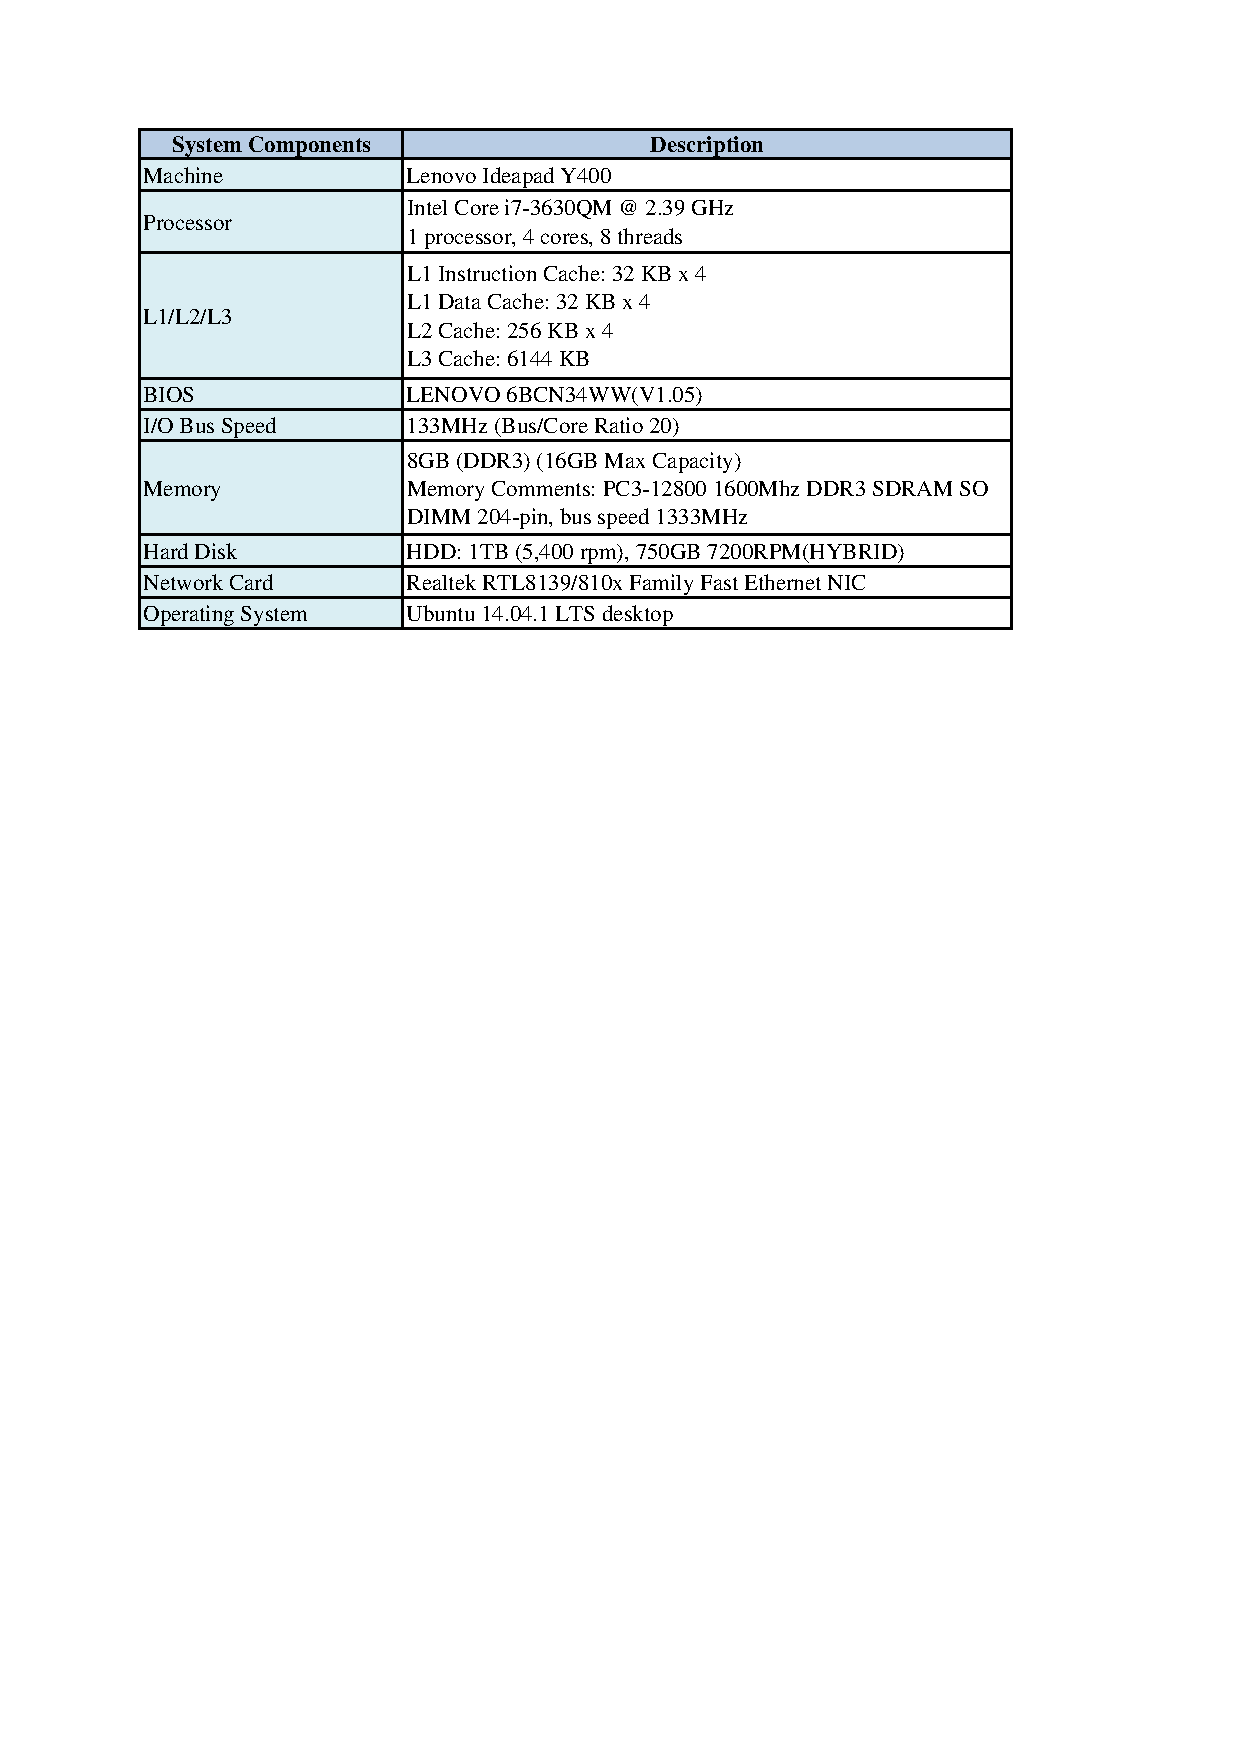
\includegraphics[width=0.4\columnwidth, angle=0]{./figs/Machine_Description.pdf}
%\caption{Machine Description of Lenovo Y400.}
%\end{figure}
%\end{comment}

\begin{figure}[!htp]
\centering
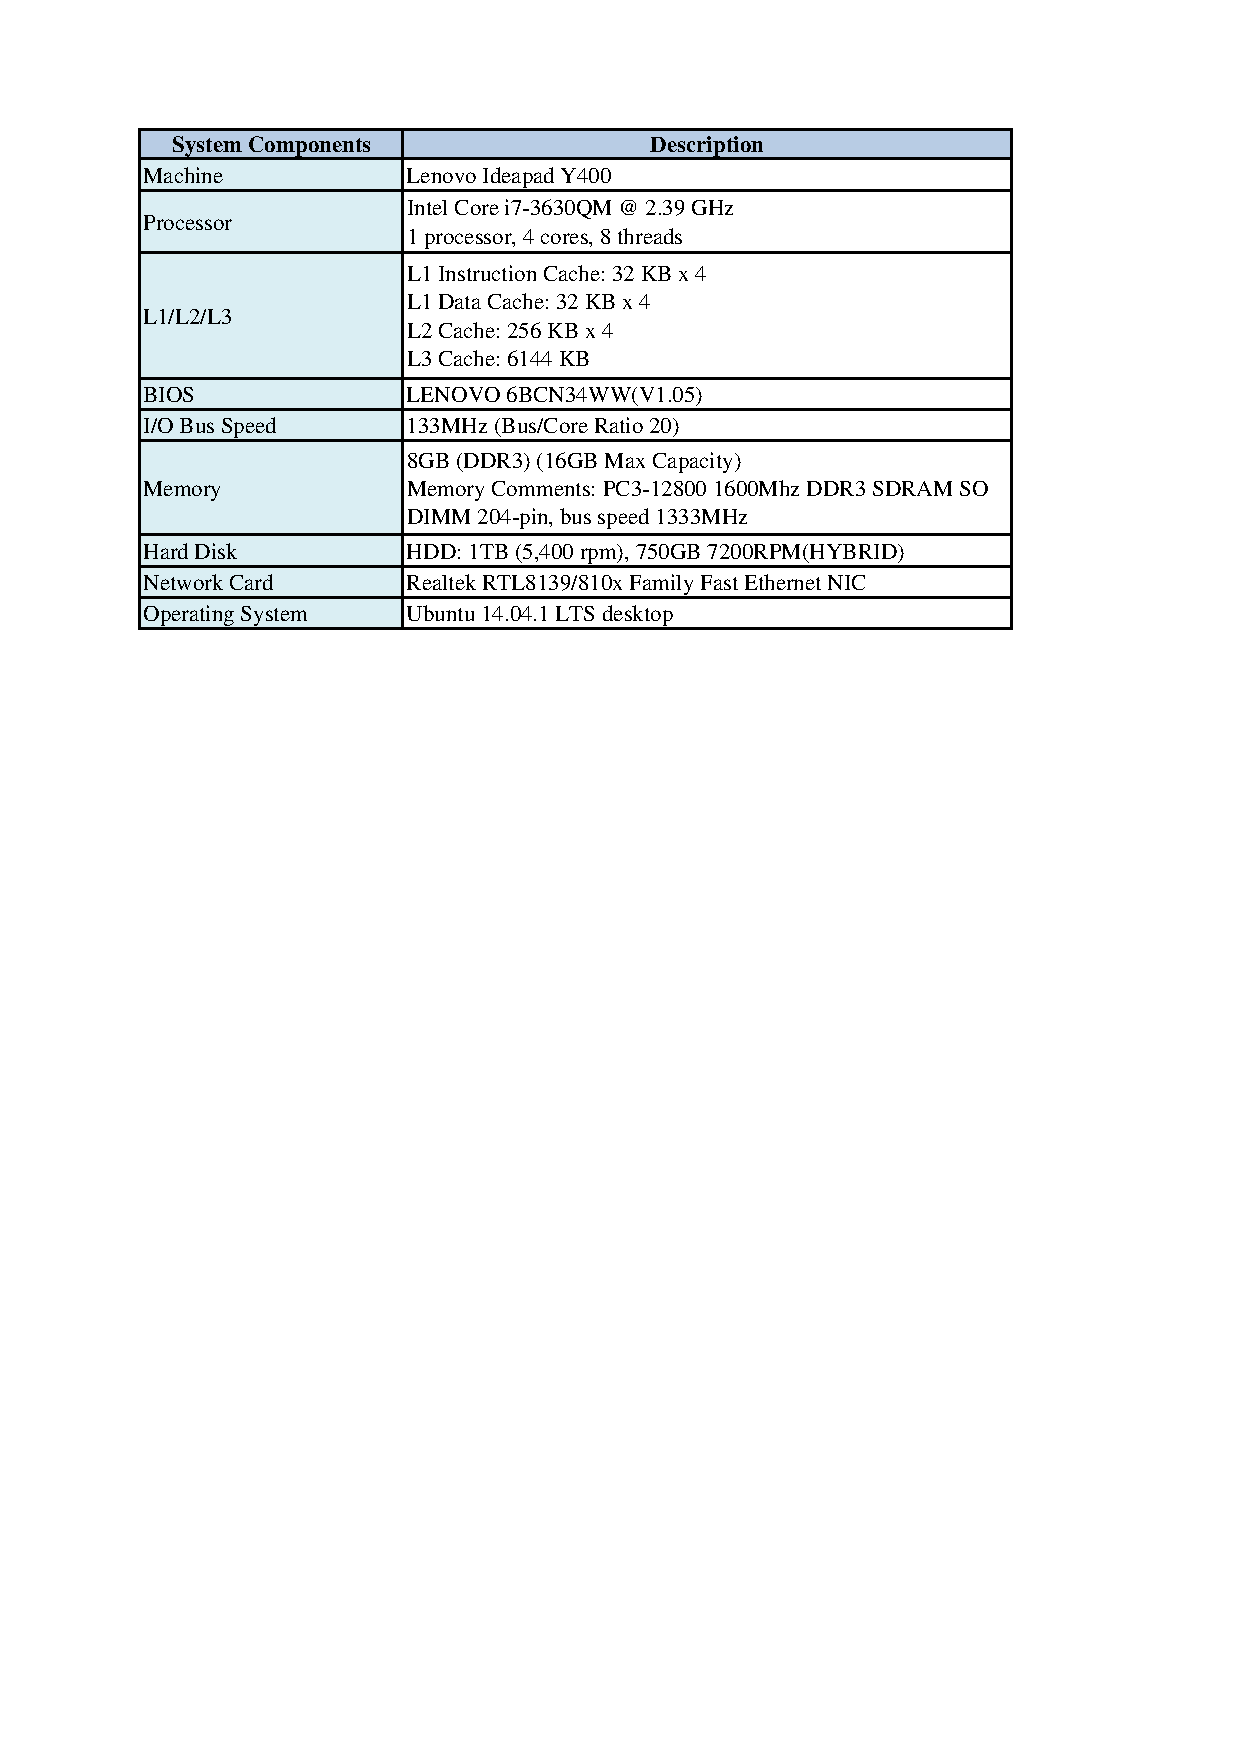
\includegraphics[width=0.5\textwidth]{figs/Machine_Description.pdf}
 \caption{Machine Description of Lenovo Y400.}
\end{figure}


\section{CPU, Scheduling, and OS Services }
\label{sec:cpu}
In this section we design several experiments to measure the performance of operations related to on-chip processor scheduling. Our experiments will provide a couple of measured results of interests.
\subsection{Measurement overhead}
\noindent\textbf{Methodology}

In order to make all the process run on single core, we will need to disable the multicore setting in bios settings. The purpose of enforcing single core is once the process runs on multicore, then the performance is not necessarily the real hardware performance.

We need to use rdtsc() as our timing stamp counter in this case in order to measure our hardware performance. rdtsc() is a function which could return the current cycle count on Intel processor. The function of rdtsc() in C++ is aligned with "inline" representation because using "inline" will reduce the function call and return overhead thereby help us get exact value of measurement overhead itself. In order to meaure the overhead of using rdtsc(), we use two consecutive rdtsc() and calculate the difference between them. And then we multiply the cycle count with the frequency of the hardware to get the overhead of the measurement. Here we use different number of iterations to see the varying of overhead.


\noindent\textbf{Predictions}

My prediction on rdtsc() measurement overhead is 65 cycle. Because rdtsc() presented in C++ is actually composed of 7 assembly instructions. According to the table listed in [1], we add the cycle counts of all 7 instructions together. Roughly, the sum of the cycle count is 65.

\noindent\textbf{Experimental Results}



\noindent\textbf{Analysis}


\subsection{Procedure call overhead}
\chunbin{Procedure call overhead: Report as a function of number of integer arguments from 0-7. What is the increment overhead of an argument?}

\noindent\textbf{Methodology}

We still use rdtsc() to calculate the cycle to measure the time. Here because we will need to examine procedure call overhead under different number of argument, we implement 8 empty functions with 0~7 argument with no return value. And then we call each function and place rdtsc() function before and after it. In order to measure the overhead more statically, we use a loop to contain the procedure call.


\noindent\textbf{Predictions}

Each procedure will have basic operations such as store, jump and return. More arguments means more store instruction for data, so more cycle counts will be applied. We predict that 5 cycles count will be applied to zero argument procudure call. If one more argument is added, then one more push instruction is needed which results to one more cycle is added.

\noindent\textbf{Experimental Results}


\noindent\textbf{Analysis}


\subsection{system call overhead}

In this part, we determine the cost of a system call that named getpid() in C++. We believe this system call has minimal cost among all of system calls because it only needs to read the process ID and return it to the user.

\noindent\textbf{Methodology}

Unlike the procedure call, the operating system caches the results of getpid(), so only the first call by a process has been executed. So we can not execute the getpid() inside a loop to get the average cost.

\noindent\textbf{Predictions}


\noindent\textbf{Experimental Results}

We have run our program 10 times,

8688, 8778,8676,7938,8670,8520,8550,8472,8556,8586

Also, we also have a program that runs getpid() ten times in a loop, and the costs are

8586, 252, 192, 196, 210, 202, 184, 192, 296, 188,

\noindent\textbf{Analysis}


\subsection{Task creation time}
In this experiment, the time of creating a new process is compared with the time of generating a kernel thread.

\noindent\textbf{Methodology}
We use the \textbf{fork()} system call and the \textbf{clone()} system call for creating a new process and a kernel thread respectively. Here we report the average cycles of $1000,000$ runs. More precisely, for fork(), to avoid the influence of extra overhead, the child process is killed immediately after each call. For clone(), we use an empty function as its input.


\noindent\textbf{Predictions}
We observe that the main operation for creating a new process is to copy resources, e.g., page tables and stack. However, lots of these resources can be shared when creating a kernel thread, e.g., the table of file descriptors. Therefore, we estimate that the time of \textit{fork()} is higher than \textit{clone()}. Because, the fork call basically makes a duplicate of the current process. Unlike fork, the clone call allow the child process to share parts of its execution context with the calling process, such as the memory space, the table of file descriptors, and the table of signal handlers \footnote{http://www.allinterview.com/showanswers/59616.html}\footnote{http://www.unixguide.net/unix/programming/1.1.2.shtml}.  Because the getPid() costs around 8000 cycles, so we predict the number of cycles for fork() and clone() is 20,000 and 16,000 respectively.

\noindent\textbf{Experimental Results}


\begin{table}[!htp]
\centering
\begin{tabular}{c|c|c}\hline\hline
 System call & Predicated value & Measured value \\
 \hline
 fork() & 20,000 & xxxx \\
 \hline
clone() & 16,000 & xxx \\ \hline\hline
\end{tabular}
\caption{Cycles for fork() and clone().}
\label{analysis:size_columndb}
\end{table}

\noindent\textbf{Analysis}

\subsection{Context switch time}
\chunbin{Context switch time: Report the time to context switch from one process to another, and from one kernel thread to another. How do they compare? In the past students have found using blocking pipes to be useful for forcing context switches}

\noindent\textbf{Methodology}

{\LinesNumberedHidden
\begin{algorithm}[htbp]
int main()$\{$\\
    pid= fork();\\
    $t_1$=rdtsc();\\
    \If{(pid==0)}
    {
        cout$<<$child timestamp :$<<$$t_1$;\\
        return 0;

    }
    \Else
    {
       $t_2$ = rdtsc();\\
        waitpid(pid);\\
        cout$<<$parent timestamp:$<<$$t_2$;\\
        return 0;
    }
$\}$
\caption{ContextSwitch}\label{FastR}
\end{algorithm}
}
\end{document}

